\documentclass[]{report}
\usepackage{graphicx, amsmath, amssymb}
\graphicspath{{/home/georg/Documents/StudyGroups/Python/naive/}}

% Title Page
\title{Parameter Learning and Prediction with Bayesian Belief Networks}
\author{Georg Heimel and Viktor Atalla}


\begin{document}
\maketitle


\begin{abstract}
Some thoughts on the matter.
\end{abstract}


\chapter{One Random Variable} \label{chap:1var}
\section{Parameter or parameter distribution?} \label{sect:set_param}
Suppose we have a single, discrete random variable $X$ with probability mass function $P(X)$. The trivial belief network illustrating this variable is shown in Fig.\,\ref{fig:1var}.
\begin{figure}[h]
	\centering
	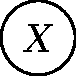
\includegraphics[scale=0.5]{1var}
	\caption{Belief network of a single, discrete random variable $X$ with probability mass function $P(X)$.}
	\label{fig:1var}
\end{figure}
Strictly speaking, this graph illustrates the situation where $P(X)$ is given in free, unparameterized form, one number for each discrete value $x$ that $X$ can take. If we want to visually represent a \emph{parameterized} probability mass function with parameter $\theta$, then we have to introduce another node for it into the graph, as shown in Fig.\,\ref{fig:1var1param}.
\begin{figure}[h]
	\centering
	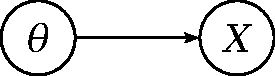
\includegraphics[scale=0.5]{1var_1param}
	\caption{A single random variable $X$, whose probability mass function is parameterized by $\theta$, which is itself a random variate.}
	\label{fig:1var1param}
\end{figure}
However, because the nodes in belief networks represent probability mass functions (or densities), not numbers, this graph represents a joint probability distribution $P(X, \theta ) $ of \emph{two} random variables, not just one. So, what we have drawn designates $\theta$ as a (usually continuous) random variate as well. Furthermore, the graph encodes a particular factorization of the joint probability distribution.
\begin{equation}
P( X, \theta)
=
P( X | \theta )
P( \theta )
\end{equation}

To recover the (now \emph{marginal}) probability mass function $P(X)$, we would have to integrate out $\theta$.
\begin{equation} \label{eq:int}
P(X)
= 
\int \mathrm{d}\theta \,
	P( X, \theta )
= 
\int\mathrm{d}\theta \,
	P( X | \theta )
	P( \theta )
\end{equation}
In oder to do that, however, we would need to know and specify the probability density $P(\theta)$. If, in contrast, we just wanted to express the concept that $P(X)$ is a probability mass function parameterized by a \emph{known}, well-defined value $\theta^*$, then we have to add one more element to the graph, as shown in Fig.\,\ref{fig:1var1param1const}.
\begin{figure}[h]
	\centering
	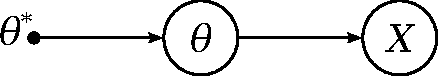
\includegraphics[scale=0.5]{1var_1param_1const}
	\caption{A single random variable $X$, whose probability mass function is parameterized by $\theta$, which is set to the number $\theta^*$.}
	\label{fig:1var1param1const}
\end{figure}
Because $\theta^*$ is a constant and no probability distribution can be assigned to it, above graph implies the following factorization of the overall joint probability.
\begin{equation} \label{eq:fact_int}
P( X, \theta )
=
P( X | \theta )
P( \theta | \theta^* )
\end{equation}
In order to \emph{set} the value of $\theta$ to $\theta^*$, we chose a \emph{delta distribution} centered on $\theta^*$ for the last term on the right-hand side.
\begin{equation} \label{eq:delta}
P( \theta | \theta^* )
=
\delta( \theta - \theta^* )
\end{equation}
Substituting \ref{eq:delta} into Eq.\,\ref{eq:fact_int} and integrating out $\theta$ yields:
\begin{equation} \label{eq:param}
P(X)
=
\int \mathrm{d}\theta \,
	P( X | \theta ) \,
	\delta( \theta - \theta^* )
= 
P( X | \theta^* )
\end{equation}
Trying to visually represent the result of this integration, \textit{i.e.}, the very right-hand side term, leads to the graph in Fig.\,\ref{fig:1var1const}. It literally spells out the parameterized probability mass function $P( X | \theta^* ) $.
\begin{figure}[h]
	\centering
	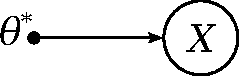
\includegraphics[scale=0.5]{1var_1const}
	\caption{A single random variable $X$, whose probability mass function is parameterized by the \emph{a priori} known and fixed number $\theta^*$.}
	\label{fig:1var1const}
\end{figure}

Returning to Eq.\,\ref{eq:int}, we could also keep $\theta$ as a random variate but chose a parameterized distribution for it as well. Calling the parameters, again fixed and known numbers, $\alpha$ and $\beta$, the graph in Fig.\,\ref{fig:1var1param2const} then encodes the factorization:
\begin{figure}[h]
	\centering
	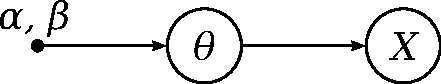
\includegraphics[scale=0.5]{1var_1param_2const}
	\caption{A single random variable $X$, whose probability mass function is parameterized by $\theta$, itself given by a distribution parameterized by $\alpha$ and $\beta$.}
	\label{fig:1var1param2const}
\end{figure}
\begin{equation} \label{eq:param prior}
P( X, \theta )
=
P( X | \theta )
P( \theta | \alpha, \beta )
\end{equation}
If we wanted, for example, to learn the distribution of $\theta$ from the distribution of $X$ with our \emph{prior} belief encoded in $P( \theta | \alpha, \beta ) $, we would factorize the left-hand side of Eq.\,\ref{eq:param prior} as $P( \theta | X ) P(X) $ and divide by $P(X)$ to arrive at:
\begin{equation} \label{eq:bayes}
P( \theta | X ) = 
\frac
	{
		P(X|\theta)
		P(\theta|\alpha, \beta)
	}
	{
		P(X)
	}
\end{equation}


\section{Learning the parameter} \label{sect:learn_param}
Clearly, if we want to predict the outcome of a future \emph{realization} of $X$, we need some idea of what the number $\theta^*$ or the probability density $P(\theta)$ should be. To learn either, we will first have to experiment and observe a number $N$ of realizations $\mathsf{x}$ of $X$ and the learned parameter (or its distribution) will depend on the specific outcome of our experiment. Trying to preserve a strict one-to-one correspondence between formulas and graphs, the repeated observations are modeled as a random process, where there are, in fact, $N$ separate random variates $X_\mathrm{i=1 \ldots N}$, all with the same probability mass function and all parameterized by the very same $\theta$, which we take to be non-parametrically distributed to keep things simple for now.

We start with a trivial factorization of the joint probability distribution of all these random variables,
\begin{equation}
{
	P( \theta | X_1, X_2, \ldots, X_\mathrm{N} )
	P( X_1, X_2, \ldots, X_\mathrm{N} )
}
=
{
	P( \theta, X_1, X_2, \ldots, X_\mathrm{N} )
}
\end{equation}
and divide by the second term on the left-hand side.
\begin{equation} \label{eq:pre_fact}
P( \theta | X_1, X_2, \ldots, X_\mathrm{N} )
=
\frac
	{
		P( \theta, X_1, X_2, \ldots, X_\mathrm{N} )
	}
	{
		P( X_1, X_2, \ldots, X_\mathrm{N} )
	}
\end{equation}

If each $X_i$ is independent of all others \emph{conditioned} on $\theta$, that is, if the observations are \textit{i.i.d}, we draw the graph for what we are about to see in our repeated experiment as shown in Fig.\,\ref{fig:1var1paramObs}; the fact that circles representing the (conditional) probability mass functions of the $X_\mathrm{i}$ are shaded indicates that these are \emph{observable} variables, while $\theta$ is a \emph{hidden} variable.
\begin{figure}[b]
	\centering
	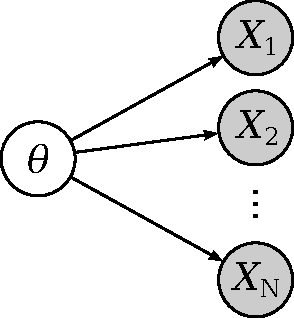
\includegraphics[scale=0.5]{1var_1param_obs}
	\caption{Multiple, independent instances of a single, observable random variable $X$, whose probability mass functions are all parameterized by the same $\theta$, which is itself a random variate, but with a non-parametric distribution.}
	\label{fig:1var1paramObs}
\end{figure}
Using the factorization implied by the graph for the joint probability distribution in the numerator of the right-hand side of Eq.\,\ref{eq:pre_fact}, we obtain:
\begin{equation} \label{eq:pre_obs}
P( \theta | X_1, X_2, \ldots, X_\mathrm{N} )
=
\frac
	{
		P(\theta)
		\prod_{i=1}^{N}
			P( X_\mathrm{i} | \theta )
	}
	{
		P( X_1, X_2, \ldots, X_\mathrm{N} )
	}
\end{equation}

Now we start our experiment and observe actual values for $X$, that is, first we observe that $X_1$ takes on the value $\mathsf{x}_1$, $X_2=\mathsf{x}_2$ and so on until we see that $X_\mathrm{N} = \mathsf{x}_\mathrm{N}$. Replacing all variables by their observed values in Eq.\,\ref{eq:pre_obs}, leads us to: 
\begin{equation} \label{eq:post_obs}
P( \theta | \mathsf{x}_1, \mathsf{x}_2, \ldots, \mathsf{x}_\mathrm{N} )
=
\frac
	{
		P( \theta )
		\prod_{i=1}^{N}
			P( \mathsf{x}_\mathrm{i} | \theta )
	}
	{
		P( \mathsf{x}_1, \mathsf{x}_2, \ldots, \mathsf{x}_\mathrm{N} )
	}
\end{equation}
The set of observed realizations $ \{ \mathsf{x}_\mathrm{i} \} $ is commonly referred to as \emph{the data}, denoted by $\mathcal{D}$. Using this notation, we finally obtain:
\begin{equation} \label{eq:learn_param}
P( \theta | \mathcal{D} )
=
\frac
	{
		P( \mathcal{D} | \theta )
		P( \theta )
	}
	{
		P( \mathcal{D} )
	}
\end{equation}

Now, given a suitable expression for $P( \mathsf{x}_i | \theta ) $ , the \emph{likelihood} of $\theta$ given the observation $\mathsf{x}_\mathrm{i}$, and a choice for the \emph{prior} probability distribution $P(\theta)$, we can learn the \emph{posterior} probability distribution of $\theta$. In general, however, computing the denominator in Eq.\,\ref{eq:learn_param}, the \emph{evidence} for the data, is quite cumbersome. Therefore, one often resorts to taking the value $\theta^*$, where the product $P( \theta | \mathcal{D} ) P( \theta ) $ has a maximum, as a \emph{point estimate} for $\theta$. Specifically, we take the \emph{maximum likelihood estimate} (MLE) if we chose a flat prior $P(\theta) = const.$
\begin{equation}
\theta_\mathrm{MLE}
=
\mathrm{argmax}_\theta\;
	P( \mathcal{D} | \theta )
\end{equation}
and the \emph{maximum posterior} (MAP) estimate if we don't.
\begin{equation}
\theta_\mathrm{MAP}
=
\mathrm{argmax}_\theta\;
	P( \mathcal{D} | \theta )
	P( \theta )
\end{equation}
Mathematically, this again corresponds to \emph{collapsing} the posterior to a delta distribution $\delta( \theta - \theta^* )$ with its center $\theta^*$ either $\theta_\mathrm{MLE}$ or $\theta_\mathrm{MAP}$. Depending on whether we do or do not chose to replace the posterior distribution with a point estimate, we end up with the graphs shown in Figs.\,\ref{fig:1var1const} and \ref{fig:1var1param}, respectively, with the difference that we now have \emph{learned} the parameter $\theta$ (or its probability density), and not just set it.

Note that, if we wanted to express our prior belief of $P(\theta)$ with a parameterized probability density, we would extend all graphs in the present Section like we demonstrated in Fig.\,\ref{fig:1var1param2const} and replace $P( \theta ) $ by $P( \theta | \alpha, \beta ) $ in all formulas accordingly (\textit{cf.} Eq.\,\ref{eq:bayes}).


\section{Predicting on new data} \label{sect:predict_new}
\subsection{The short answer}
We can now proceed to predict the probability mass function for the outcome of a new realization of our univariate random process. To distinguish this event from past observations, we introduce yet another random variate, $X^*$ this time. Now, if we chose a (learned) point estimate $\theta^*$ for the parameter of the probability mass function (\textit{e.g.}, MLE or MAP), we have to look no further than Fig.\,\ref{fig:1var1const} and Eq.\,\ref{eq:param}.
\begin{equation}
P( X^* )
=
P( X^* | \theta^* )
\end{equation}
If, however, we decided to keep the entire posterior distribution of $\theta$, then we are in the situation depicted in Fig.\,\ref{fig:1var1param} and, consequently, have to employ Eq.\,\ref{eq:int}.
\begin{equation}
P(X^*)
=
\int \mathrm{d}\theta \,
	P( X^* | \theta )
	P( \theta )
\end{equation}


\subsection{The long answer}
To explicitly express that $P(\theta)$ is indeed our \emph{posterior} belief about the distribution of $\theta$, and that we are indeed predicting the probability mass function for a new observation \emph{after} having seen the data, we explicitly introduce $X^*$ into the graph in Fig.\,\ref{fig:1var1paramObs} to produce the one shown in Fig.\,\ref{fig:1var1paramNewObs}.
\begin{figure}[h]
	\centering
	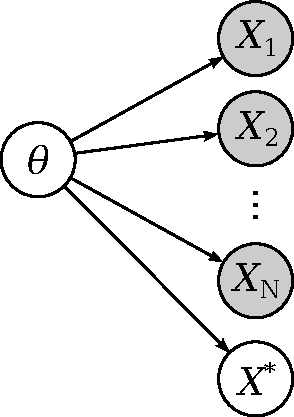
\includegraphics[scale=0.5]{1var_1param_new-obs}
	\caption{Same as Figure\,\ref{fig:1var1paramObs} with $X^*$ representing a new, unobserved instance of $X$.}
	\label{fig:1var1paramNewObs}
\end{figure}
Collecting all the $X_\mathrm{i}$ as $\mathcal{D}$, the joint probability of all three parameters $X^*$, $\theta$, and $\mathcal{D}$, can then be factorized in two ways which are, of course, equal to each other. Specifically, we chose:
\begin{equation}
P( X^*, \theta | \mathcal{D} )
P (\mathcal{D} )
=
P( X^*, \mathcal{D} | \theta )
P( \theta )
\end{equation}
Because all observations of $X$, past or future, are independent of each other conditioned on $\theta$, $X^*$ is also independent from $\mathcal{D}$. We can, therefore, rewrite the right-hand side,
\begin{equation}
P( X^*, \theta | \mathcal{D} )
P( \mathcal{D} )
= 
P( X^* | \theta )
P( \mathcal{D} | \theta )
P( \theta )
\end{equation}
join its last two terms,
\begin{equation}
P( X^*, \theta | \mathcal{D} )
P( \mathcal{D} )
= 
P( X^* | \theta )
P( \mathcal{D}, \theta )
\end{equation}
take them apart again the other way around,
\begin{equation}
P( X^*, \theta | \mathcal{D} )
P( \mathcal{D} ) 
= 
P( X^* | \theta )
P( \theta | \mathcal{D} )
P( \mathcal{D} )
\end{equation}
and divide by $P(\mathcal{D})$.
\begin{equation}
P( X^*, \theta | \mathcal{D} ) 
= 
P( X^* | \theta )
P( \theta | \mathcal{D} )
\end{equation}
Now integrating over $\theta$ brings us to the formal expression for the \emph{posterior predictive}.
\begin{equation} \label{eq:post_pred}
P( X^* | \mathcal{D} ) 
= 
\int \mathrm{d}\theta \,
	P( X^* | \theta )
	P( \theta | \mathcal{D} )
\end{equation}


\chapter{Two Random Variables}
\section{Repeat after me ...} \label{sect:d-connect}
Let $\mathcal{X}$, $\mathcal{Y}$, and $\mathcal{Z}$ be three non-intersecting sets of nodes in the directed graph $G$, that is $\mathcal{X}\cap\mathcal{Y} = \mathcal{X}\cap\mathcal{Z} = \mathcal{Y}\cap\mathcal{Z} = \varnothing$. We define
$\mathcal{X}$ and $\mathcal{Y}$ to be $d$-separated by $\mathcal{Z}$ in $G$ iff all paths between every $x \in \mathcal{X}$ and every $y \in \mathcal{Y}$ are \emph{blocked}. A path $U$ is said to be blocked iff there is a node $w$ on $U$ such that either
\begin{itemize}
	\item $w$ is a collider and neither $w$ nor any of its descendants is in $\mathcal{Z}$, or
	\item $w$ is not a collider on $U$ and $w$ is in $\mathcal{Z}$.
\end{itemize}
If, in particular, $G$ represents a \emph{belief network} and, thus, the nodes represent random variates, then $\mathcal{X}$ and $\mathcal{Y}$ are independent conditional on $\mathcal{Z}$ in all probability distributions $G$ can represent iff $\mathcal{X}$ and $\mathcal{Y}$ are $d$-separated by $\mathcal{Z}$.


\section{Parameter separation} \label{sect:param-sep}
Moving on, we now suppose we have two random variables, $X$ and $Y$, parameterized by $\theta_\mathrm{x}$ and $\theta_\mathrm{y}$, respectively. To make things more interesting, we will further suppose that they are not independent of each other but that, on the contrary, the value that $X$ takes impacts the distribution of values observed for $Y$. Because our distributions are parameterized, affecting the probability mass function of $Y$ means affecting the parameter $\theta_\mathrm{y}$ that defines it. The graph encoding the situation just described, shown in Fig.\,\ref{fig:2var2param}, suggest the following factorization of the joint distribution of all involved random variates.
\begin{figure}[h]
	\centering
	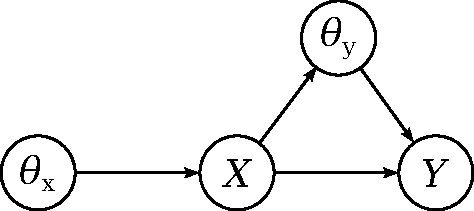
\includegraphics[scale=0.5]{2var_2param}
	\caption{Two correlated random variables, $X$ and $Y$, with their probability mass functions parameterized by $\theta_\mathrm{x}$ and $\theta_\mathrm{y}$, which are themselves random variables, but with non-parametric distributions.}
	\label{fig:2var2param}
\end{figure}
\begin{equation} \label{eq:2param_from_G}
P( Y, X, \theta_\mathrm{y}, \theta_\mathrm{x} )
= 
P( Y | \theta_\mathrm{y}, X )
P( \theta_\mathrm{y} | X )
P( X | \theta_\mathrm{x} )
P( \theta_\mathrm{x} )
\end{equation}
In an attempt to find a second, complementary factorization that would allow us to find the analogue to Eq.\,\ref{eq:learn_param} for two parameters, we start by conditioning on $X$.
\begin{equation}
P( Y, \theta_\mathrm{y}, \theta_\mathrm{x} | X )
P( X ) 
=
rhs
\end{equation}
Using the recipe from Section\,\ref{sect:d-connect}, we then realize that both $Y$ and $\theta_\mathrm{y}$ are independent of $\theta_\mathrm{x}$ conditioned on $X$ (because $X$ is on any path between them, is \emph{not} a collider, and \emph{is} in the conditioning set).
\begin{equation}
P( Y, \theta_\mathrm{y} | X )
P( \theta_\mathrm{x} | X )
P( X ) 
= 
rhs
\end{equation}
Next, we combine the lone $P(X)$ with the first factor,
\begin{equation}
P( Y, X, \theta_\mathrm{y} )
P( \theta_\mathrm{x} | X ) 
= 
rhs
\end{equation}
and tear that factor apart in a different way.
\begin{equation} \label{eq:2param_lhs}
P( \theta_\mathrm{y} | Y, X )
P( Y, X )
P( \theta_\mathrm{x} | X ) 
= 
rhs
\end{equation}
Writing out again the right-hand side of Eq.\,\ref{eq:2param_from_G} and dividing by $P(Y, X) = P(Y|X) P(X)$ then yields:
\begin{equation} \label{eq:2param_prod}
P( \theta_\mathrm{y} | Y, X )
P( \theta_\mathrm{x} | X ) 
= 
\frac
	{
		P( Y | \theta_\mathrm{y}, X )
		P( \theta_\mathrm{y} | X )
		P( X | \theta_\mathrm{x} )
		P( \theta_\mathrm{x} )
	}
	{
		P( Y | X )
		P( X )
	}
\end{equation}
Comparing this to Eq. \ref{eq:learn_param}, we see that we got what we asked for, sort of. But how are we going to learn the parameters $\theta_\mathrm{x}$ and $\theta_\mathrm{y}$ at the same time? The answer is, we aren't because Eq.\,\ref{eq:2param_prod} is actually the product of two equations, one for each parameter, and we need to separate it to learn them one by one.

First, we combine the last to terms in the numerator on the right-hand side of Eq.\,\ref{eq:2param_prod} to $P(\theta_\mathrm{x}, X)$ and take that apart the other way around.
\begin{equation}
P( \theta_\mathrm{y} | Y, X )
P( \theta_\mathrm{x} | X ) 
= 
\frac
	{
		P( Y | \theta_\mathrm{y}, X )
		P( \theta_\mathrm{y} | X )
		P( \theta_\mathrm{x} | X )
		P( X )
	}
	{
		P( Y | X )
		P( X )
	}
\end{equation}
Then we realize that the newly created factors cancel with existing ones only to yield,
\begin{equation} \label{eq:2param_Y}
P( \theta_\mathrm{y} | Y, X ) 
= 
\frac
	{
		P( Y | \theta_\mathrm{y}, X )
		P( \theta_\mathrm{y} | X )
	}
	{
		P( Y | X )
	}
\end{equation}
which we recognize as the "first half" of Eq.\,\ref{eq:2param_prod}. We will use this expression to learn the $X$-dependent parameter $\theta_\mathrm{y}$.

To isolate an equivalent expression for $\theta_\mathrm{x}$, we start again with Eq.\,\ref{eq:2param_prod} and multiply with $P(X)$,
\begin{equation}
P( \theta_\mathrm{y} | Y, X )
P( X )
P( \theta_\mathrm{x} | X ) 
= 
\frac
	{
		P( Y |\theta_\mathrm{y}, X )
		P( \theta_\mathrm{y} | X )
		P( X )
		P( X | \theta_\mathrm{x} )
		P( \theta_\mathrm{x} )
	}
	{
		P( Y | X )
		P( X )
	}
\end{equation}
combine the first three terms in the numerator on the right-hand side,
\begin{equation}
P( \theta_\mathrm{y} | Y, X )
P( X )
P( \theta_\mathrm{x} | X ) 
=
\frac
	{
		P( Y, X, \theta_\mathrm{y} )
		P( X | \theta_\mathrm{x} )
		P( \theta_\mathrm{x} )
	}
	{
		P( Y | X )
		P( X )
	}
\end{equation}
multiply by $P(Y|X)$,
\begin{equation}
P( \theta_\mathrm{y} | Y, X )
P( Y | X )
P( X )
P( \theta_\mathrm{x} | X ) 
= 
\frac
	{
		P( Y, X, \theta_\mathrm{y} )
		P( X | \theta_\mathrm{x} )
		P( \theta_\mathrm{x} )
	}
	{
		P( X )
	}
\end{equation}
and combine the first three terms on the left-hand side, 
\begin{equation}
P( Y, X, \theta_\mathrm{y} )
P( \theta_\mathrm{x} | X ) 
= 
\frac
	{
		P( Y, X, \theta_\mathrm{y} )
		P( X | \theta_\mathrm{x} )
		P( \theta_\mathrm{x} )
	}
	{
		P( X )
	}
\end{equation}
which cancel with their right-hand side equivalent to give us,
\begin{equation}
P( \theta_\mathrm{x} | X ) 
=
\frac
	{
		P( X | \theta_\mathrm{x} )
		P( \theta_\mathrm{x} )
	}
	{
		P( X )
	}
\end{equation} \label{eq:2param_X}
which we recognize as the "second half" of Eq.\,\ref{eq:2param_prod}.


\section{Learning the parameters}
\subsection{The short answer}
Looking at Eq.\,\ref{eq:2param_X}, we realize that we can proceed in exactly the same manner as for the univariate case discussed in Section\,\ref{sect:learn_param} to learn the parameter $\theta_\mathrm{x}$. We denote the obtained posterior $P( \theta_\mathrm{x} | \mathcal{D}_\mathrm{x} ) $ because we do not, in fact, need the values observed for $Y$ to learn $\theta_\mathrm{x}$, but only the set $\{\mathsf{x}_\mathrm{i}\} = \mathcal{D}_\mathrm{x}$ of realizations of $X$. To learn $\theta_\mathrm{y}$, we take another look at Eq.\,\ref{eq:2param_Y} and realize that everything is conditioned on $X$, by definition a \emph{discrete} random variable that can take on the values $x_1, x_2, \ldots$ So, instead of just one equation, we are actually looking at as many as there are different values for $X$.
\begin{align}
P( \theta_\mathrm{y} | Y, X = x_1 )
&= 
\frac
	{
		P( Y | \theta_\mathrm{y}, X = x_1 )
		P( \theta_\mathrm{y} | X = x_1 )
	}
	{
		P( Y | X = x_1 )
	}
\nonumber \\
P( \theta_\mathrm{y} | Y, X = x_2 )
&=
\frac
	{
		P( Y | \theta_\mathrm{y}, X = x_2 )
		P( \theta_\mathrm{y} | X = x_2 )
	}
	{
		P( Y | X=x_2 )
	}
\\
&\vdots
\nonumber
\end{align}
This suggest that, having collected paired realizations of $X$ and $Y$, we group by the possible values of $X$, specify a prior $P( \theta_\mathrm{y} | X ) $ for each of them, and compute a separate posterior for $\theta_\mathrm{y}$ from the $Y$ realizations in each group, again following Section\,\ref{sect:learn_param}.


\subsection{The long answer}
Let's start by staring at Eq.\,\ref{eq:2param_Y} yet again.
\begin{equation*}
P( \theta_\mathrm{y} | Y, X ) 
=
\frac
	{
		P( Y | \theta_\mathrm{y}, X )
		P( \theta_\mathrm{y} | X )
	}
	{
		P( Y | X )
	}
\end{equation*}
It was derived by rigorously applying the rules for manipulating probability distributions but, to actually use it, we now must understand just what each term really means. Starting with the first of the two factors in the numerator, we acknowledge that it gives us the possibility to specify a different likelihood for each value $x$ that $X$ can take. While we might not actually want to do that, we still note that the product
\begin{equation} \label{eq:2param_likelihood_Y}
P( Y | \theta_\mathrm{y}, X ) 
=
\prod_{k}
	{
		p_\mathrm{k}( Y | \theta_\mathrm{y} )
	}
	^
	{
		[ X = x_\mathrm{k} ]
	}
\end{equation} 
does the trick of filtering out the likelihood $p_\mathrm{k}( Y | \theta_\mathrm{y} ) $ by setting $X$ to $x_\mathrm{k}$. This is thanks to the \emph{Iverson bracket} in the exponent, which evaluates to 1 if its contents are true and to 0 otherwise.

Likewise, the second term in the numerator intuitively expresses that a different prior $\pi( \theta_\mathrm{y} ) $ can be chosen for every value $x$ that $X$ can take. This is again expressed in the same way,
\begin{equation} \label{eq:2param_prior_Y}
P( \theta_\mathrm{y} | X ) 
=
\prod_{k}
	{
		\pi_\mathrm{k}( \theta_\mathrm{y} )
	}
	^
	{
		[ X = x_\mathrm{k} ]
	}
\end{equation}
which yields for the entire numerator:
\begin{equation}
P( Y | \theta_\mathrm{y}, X )
P( \theta_\mathrm{y} | X ) 
=
\prod_{k}
	\Bigl\{
		p_\mathrm{k}( Y | \theta_\mathrm{y} )
		\pi_\mathrm{k}( \theta_\mathrm{y} )
	\Bigr\}
	^
	{
		[ X = x_\mathrm{k} ]
	}
\end{equation}
Finally, the denominator is the integral of the numerator over $\theta_\mathrm{y}$.
\begin{align}
P(Y|X)
&=
\int \mathrm{d}\theta_\mathrm{y}
	\prod_{k}
		\Bigl\{
			p_\mathrm{k}( Y | \theta_\mathrm{y} )
			\pi_\mathrm{k}( \theta_\mathrm{y} )
		\Bigr\}
		^
		{
			[ X = x_\mathrm{k} ]
		}
\nonumber \\ 
&=
\prod_{k}
	\left\{
		\int \mathrm{d}\theta_\mathrm{y} \,
			p_\mathrm{k}( Y | \theta_\mathrm{y} )
			\pi_\mathrm{k}( \theta_\mathrm{y} )
	\right\}
	^
	{
		[ X = x_\mathrm{k} ]
	}
\\
&\stackrel{!}{=}
\prod_{k}
	{
		p_\mathrm{k}( Y )
	}
	^
	{
		[ X = x_\mathrm{k} ]
	}
\nonumber
\end{align}
Putting it all together, then leads us to realize that the conditional posterior
\begin{align}
P( \theta_\mathrm{y} |Y, X ) 
&=
\prod_{k}
	\left\{
		\frac
			{
				p_\mathrm{k}( Y | \theta_\mathrm{y} )
				\pi_\mathrm{k}( \theta_\mathrm{y} )
			}
			{
				p_\mathrm{k}( Y )
			}
	\right\}
	^
	{
		[ X = x_\mathrm{k} ]
	}
\nonumber \\
&\stackrel{!}{=}
\prod_{k}
	{
		p_\mathrm{k}( \theta_\mathrm{y} | Y )
	}
	^
	{
		[ X = x_\mathrm{k} ]
	}
\end{align}
is actually a product of as many posteriors as there a values that $X$ can take. Our goal, of course, is to learn every single one of them.


\subsubsection{Extending the graph}
Having grasped the multitude of posteriors we want to learn as well as their functional relationships, we now take a step back, and extend the graph in Fig.\,\ref{fig:2var2param} as we did in Section\,\ref{sect:learn_param} to include multiple instances of the two random variates that are to be observed.
\begin{figure}[h]
	\centering
	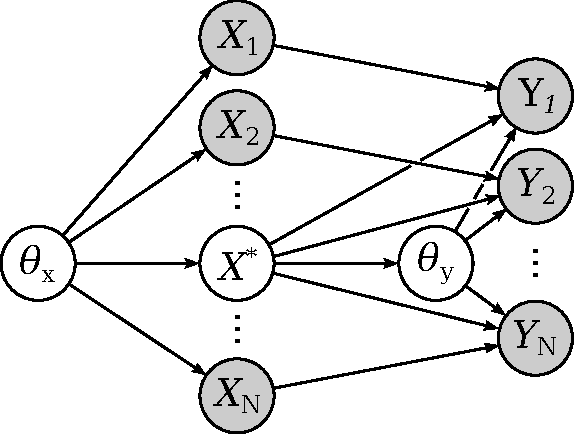
\includegraphics[scale=0.5]{2var_2param_obs}
	\caption{Multiple, independent instances of two correlated random variables, $X$ and $Y$, with their probability mass functions parameterized by $\theta_\mathrm{x}$ and $\theta_\mathrm{y}$, which are themselves random variables, but with non-parametric distributions.}
	\label{fig:2var2paramObs}
\end{figure}
Note that the monstrosity in Fig.\,\ref{fig:2var2paramObs} seems to lie somewhere between Figs.\,\ref{fig:1var1paramObs} and \ref{fig:1var1paramNewObs}. We will see soon enough that the extra, unobserved $X$ is necessary to capture the conditional dependence of the posterior in $\theta_\mathrm{y}$.

This graph then encodes the following factorization of the joint probability of all involved variables (\textit{cf.} Eq.\,\ref{eq:2param_from_G}):
\begin{equation}
lhs 
= 
\left\{
	\prod_{i=1}^{N}
		P( Y_\mathrm{i} | \theta_\mathrm{y}, X_\mathrm{i}, X^* )
\right\}
P( \theta_\mathrm{y} | X^* )
\left\{
	\prod_{i=1}^{N}
		P( X_\mathrm{i} | \theta_\mathrm{x} )
\right\}
P( X^* | \theta_\mathrm{x} ) \,
P( \theta_\mathrm{x} )
\end{equation}
To find the matching left-hand side, we first redo the exact same derivation as in Section\,\ref{sect:param-sep}, with the entire set of all $\{Y_\mathrm{i}\}$ taking the place of the lone $Y$ and, likewise, the entire set of all $\{X_\mathrm{i}\}$ plus the $X^*$ substituted for the lone $X$. This first leads us to the equivalent of Eq.\,\ref{eq:2param_lhs}.
\begin{equation}
P( \theta_\mathrm{y} | \{Y_\mathrm{i}\}, \{X_\mathrm{i}\}, X^* ) \,
P( \theta_\mathrm{x} | \{X_\mathrm{i}\}, X^* ) \,
P( \{Y_\mathrm{i}\}, \{X_\mathrm{i}\}, X^* )
= 
rhs
\end{equation}
Also the next step is analogous to the preceding Section\,\ref{sect:param-sep} in that we factorize the last term into $P( \{ Y_\mathrm{i} \} | \{ X_\mathrm{i} \}, X^* ) \, P( \{ X_\mathrm{i} \}, X^* ) $, which allows us again to separate into two parts.
\begin{equation} \label{eq:2params_obs_Y}
P( \theta_\mathrm{y} | \{Y_\mathrm{i}\}, \{X_\mathrm{i}\}, X^* ) 
=
\frac
	{
		P( \theta_\mathrm{y} | X^* )
		\prod_{i=1}^{N}
			P( Y_\mathrm{i} | \theta_\mathrm{y}, X_\mathrm{i}, X^*)
	}
	{
		P( \{Y_\mathrm{i}\} | \{X_\mathrm{i}\}, X^* )
	} 
\end{equation}
\begin{equation} \label{eq:2params_obs_X}
P( \theta_\mathrm{x} | \{X_\mathrm{i}\}, X^* ) 
=
\frac
	{
		P( X^* | \theta_\mathrm{x} )
		P( \theta_\mathrm{x} )
		\prod_{i=1}^{N}
			P( X_\mathrm{i} | \theta_\mathrm{x} )
	}
	{
		P( \{X_\mathrm{i}\}, X^* )
	} 
\end{equation}

\subsubsection{Posterior of $\theta_\mathrm{x}$}
The appearance of the auxiliary quantity $X$ in Eq.\,\ref{eq:2params_obs_X} is sitting somewhat oddly in the above expression for the posterior of $\theta_\mathrm{x}$. Why should one of the instances of $X$ stick out from the rest? Fortunately, it is not hard to make it disappear. To do so, we multiply with the denominator of the right-hand side,
\begin{equation}
P( \theta_\mathrm{x}, \{X_\mathrm{i}\}, X^* ) 
=
P( X^* | \theta_\mathrm{x} ) \,
P( \theta_\mathrm{x} )
\prod_{i=1}^{N}
	P (X_\mathrm{i} | \theta_\mathrm{x} )
\end{equation}
and pluck apart the left-hand side by conditioning on $\theta_\mathrm{x}$.
\begin{equation}
P( \{X_\mathrm{i}\}, X^* | \theta_\mathrm{x} ) \,
P( \theta_\mathrm{x} )
= 
rhs
\end{equation}
Examining the graph in Fig.\,\ref{fig:2var2paramObs} in the light of Section\,\ref{sect:d-connect}, we realize that paths from $X^*$ to any of the $ \{ X_\mathrm{i} \} $ either lead us through $\theta_\mathrm{x}$, which is not a collider but is in the conditioning set, or through one of the $\{Y_\mathrm{i}\}$, which are all colliders and are not in the conditioning set. Thus, all these paths are blocked and we can further write:  
\begin{align}
P( \{X_\mathrm{i}\} | \theta_\mathrm{x} ) \,
P( X^* | \theta_\mathrm{x} ) \,
P( \theta_\mathrm{x} )
&=
rhs
\nonumber \\
P( \theta_\mathrm{x}, \{X_\mathrm{i}\} ) \,
P( X^* | \theta_\mathrm{x} )
&= 
rhs
\\
P( \theta_\mathrm{x} | \{X_\mathrm{i}\} ) \,
P( \{X_\mathrm{i}\} ) \,
P( X^* | \theta_\mathrm{x} )
&= 
rhs
\nonumber
\end{align}
Now that we see how the offensive term $P( X^* | \theta_\mathrm{x} ) $ cancels with its equivalent on the right-hand side, we can divide again by $P( \{X_\mathrm{i}\} ) $ and replace the variables by their realizations $ \{ \mathsf{x}_\mathrm{i} \} $ to arrive at:
\begin{equation}
P( \theta_\mathrm{x} | \{ \mathsf{x}_\mathrm{i} \} ) 
=
\frac
	{
		P( \theta_\mathrm{x} )
		\prod_{i=1}^{N}
			P( \mathsf{x}_\mathrm{i} | \theta_\mathrm{x} )
	}
	{
		P( \{ \mathsf{x}_\mathrm{i} \} )
	} 
\end{equation}
If we denote, as before, $ \{ \mathsf{x}_\mathrm{i} \} = \mathcal{D}_\mathrm{x}$, we finally end up with the familiar expression for the posterior of $\theta_\mathrm{x}$.
\begin{equation}
P( \theta_\mathrm{x} | \mathcal{D}_\mathrm{x} ) 
= 
\frac
	{
		P( \mathcal{D}_\mathrm{x} | \theta_\mathrm{x} )
		P( \theta_\mathrm{x} )
	}
	{
		P( \mathcal{D}_\mathrm{x} )
	} 
\end{equation}

\subsubsection{Posterior(s) of $\theta_\mathrm{y}$}
To make sense of Eq.\,\ref{eq:2params_obs_Y}, we first plug Eqs.\,\ref{eq:2param_likelihood_Y} and \ref{eq:2param_prior_Y} into the numerator ($num$) of the right-hand side,
\begin{align}
num 
&=
\prod_{k}
	{
		\pi_\mathrm{k}( \theta_\mathrm{y} )
	}
    ^
    {
		[ X^* = x_\mathrm{k} ]
	}
\prod_{i=1}^{N}
	\left\{
		\prod_{k}
			{
				p_\mathrm{k}( Y_\mathrm{i} | \theta_\mathrm{y} )
			}
		    ^
		    {
				[ X_\mathrm{i} = x_\mathrm{k} ]
			}
	\right\}
	^
	{
		[ X_\mathrm{i} = X^* ]
	}
\nonumber \\
&=
\prod_{k}
	{
		\pi_\mathrm{k}( \theta_\mathrm{y} )
	}
    ^
    {
		[ X^* = x_\mathrm{k} ]
	}
\prod_{k}
	\left\{
		\prod_{i=1}^{N}
			{
				p_\mathrm{k}( Y_\mathrm{i} | \theta_\mathrm{y} )
			}
			^
			{
				[ X_\mathrm{i} = x_\mathrm{k} ]
			}
	\right\}
	^
	{
		[ X^* = x_\mathrm{k} ]
	}
\nonumber \\
&=
\prod_{k}
	\left\{
		\pi_\mathrm{k}( \theta_\mathrm{y} )
		\prod_{i=1}^{N}
			{
				p_\mathrm{k}( Y_\mathrm{i} |\theta_\mathrm{y} )
			}
			^
			{
				[ X_\mathrm{i} = x_\mathrm{k} ]
			}
	\right\}
	^
	{
		[ X^* = x_\mathrm{k} ]
	}
\nonumber \\
&\stackrel{!}{=}
\prod_{k}
	\Bigl\{
		p_\mathrm{k}
			\bigl(
				\left\{ Y_\mathrm{i} | X_\mathrm{i} = x_\mathrm{k} \right\} |
				\theta_\mathrm{y}
			\bigr) \,
		\pi_\mathrm{k}( \theta_\mathrm{y} )
	\Bigr\}
	^
	{
		[ X^* = x_\mathrm{k} ]
	}
\end{align}
which leaves us with
\begin{align}
den 
&= 
\prod_{k}
	\left\{
		\int \mathrm{d}\theta_\mathrm{y} \,
			\pi_\mathrm{k}( \theta_\mathrm{y} )
			\prod_{i=1}^{N}
				{
					p_\mathrm{k}( Y_\mathrm{i} | \theta_\mathrm{y} )
				}
				^
				{
					[ X_\mathrm{i} = x_\mathrm{k} ]
				}
	\right\}
	^
	{
		[ X^* = x_\mathrm{k} ]
	} 
\nonumber \\
&\stackrel{!}{=}
\prod_{k}
	\Bigl\{
		p_\mathrm{k}
			\bigl(
			\left\{ Y_\mathrm{i} | X_\mathrm{i} = x_\mathrm{k} \right\}
			\bigr)
	\Bigr\}
	^
	{
		[ X^* = x_\mathrm{k} ]
	}
\end{align}
for the denominator ($den$). Putting it all together and substituting the actual realizations, $ \{ \mathsf{y}_\mathrm{i} \} $ and $ \{ \mathsf{x}_\mathrm{i} \} $, of $Y$ and $X$, respectively, we then arrive at:
\begin{align}
P( \theta_\mathrm{y} | \{ \mathsf{y}_\mathrm{i} \}, \{ \mathsf{x}_\mathrm{i} \}, X^*) 
&=
\prod_{k}
	\left\{
		\frac
			{
				p_\mathrm{k}
					\bigl(
						\left\{ 
							\mathsf{y}_\mathrm{i} | 
							\mathsf{x}_\mathrm{i} = x_\mathrm{k}
						\right\} |
						\theta_\mathrm{y}
					\bigr)
				\pi_\mathrm{k}( \theta_\mathrm{y} )
			}
			{
				p_\mathrm{k}
					\bigl(
						\left\{
							\mathsf{y}_\mathrm{i} | 
							\mathsf{x}_\mathrm{i} = x_\mathrm{k}
						\right\} 
					\bigr)
			}
	\right\}
	^
	{
		[ X^* = x_\mathrm{k} ]
	}
\nonumber \\
&\stackrel{!}{=}
\prod_{k}
	\Bigl\{
		p_\mathrm{k}
			\bigl(
				\theta_\mathrm{y} |
				\left\{
					\mathsf{y}_\mathrm{i} |
					\mathsf{x}_\mathrm{i} = x_\mathrm{k}
				\right\}
			\bigr)
	\Bigr\}
	^
	{
		[ X^* = x_\mathrm{k} ]
	} 
\end{align}
Introducing $\mathcal{D}_\mathrm{y}^{\,k} = \{ \mathsf{y}_\mathrm{i} | \mathsf{x}_\mathrm{i} = x_\mathrm{k} \} $, we could also rewrite this as,
\begin{equation}
P( \theta_\mathrm{y} | \mathcal{D}, X^* ) 
=
\prod_{k}
	\Bigl\{
		p_\mathrm{k}( \theta_\mathrm{y} | \mathcal{D}_\mathrm{y}^{\,k} )
	\Bigr\}
	^
	{
		[ X^* = x_\mathrm{k} ]
	}
\end{equation}
where the relevant factors are given by:
\begin{equation}
p_\mathrm{k}( \theta_\mathrm{y} | \mathcal{D}_\mathrm{y}^{\,k} ) 
=
\frac
	{
		p_\mathrm{k}( \mathcal{D}_\mathrm{y}^{\,k} | \theta_\mathrm{y} )
		\pi_\mathrm{k}( \theta_\mathrm{y} )
	}
	{
		p_\mathrm{k}( \mathcal{D}_\mathrm{y}^{\,k} )
	}
\end{equation}

\section*{Proceed at your own risk from here!}
\section{Predicting on new data}
To predict the probability mass function for a new observation $X^*$, we proceed in exactly the same way as for the single-variable case outlined in Section\,\ref{sect:predict_new} and rewrite Eq.\,\ref{eq:post_pred}.
\begin{equation} \label{eq:post_pred_X}
P( X^* | \mathcal{D}_\mathrm{x} )
= 
\int \mathrm{d}\theta_\mathrm{x} \,
	P( X^* | \theta_\mathrm{x} )
	P( \theta_\mathrm{x} | \mathcal{D}_\mathrm{x} )
\end{equation}
The same is true if we wanted to predict the probability mass function for a new observation $Y^*$ given a certain value of $X^*$.
\begin{equation} \label{eq:post_pred_Y}
P(Y^*|X^*, \mathcal{D}) = \int\mathrm{d}\theta_\mathrm{y}\,P(Y^*|\theta_\mathrm{y}, X^*)P(\theta_\mathrm{y}|\mathcal{D}, X^*)
\end{equation}
Again, Eq.\,\ref{eq:post_pred_Y} is actually many equations, one for every value $x^*$ that $X^*$ can take. Multiplying with Eq.\,\ref{eq:post_pred_X},
\begin{equation}
P(Y^*, X^*|\mathcal{D}) = P(Y^*|X^*, \mathcal{D})P(X^*|\mathcal{D})
\end{equation}
we get the joint posterior predictive,
\begin{equation} \label{eq:post_pred_joint}
P(Y^*, X^*|\mathcal{D}) = \int\mathrm{d}\theta_\mathrm{y}\mathrm{d}\theta_\mathrm{x}\,P(Y^*|\theta_\mathrm{y}, X^*)P(\theta_\mathrm{y}|\mathcal{D}, X^*)P(X^*|\theta_\mathrm{x})P(\theta_\mathrm{x}|\mathcal{D})
\end{equation}
and that for a new observation $X^*$ given a certain value of $Y^*$.
\begin{equation} \label{eq:post_pred_XY}
P(X^*|Y^*, \mathcal{D}) = \frac{P(Y^*, X^*|\mathcal{D})}{P(Y^*|\mathcal{D})}
\end{equation}
The denominator on the right-hand side of this expression is obtained by summing the joint posterior predictive in Eq.\,\ref{eq:post_pred_joint} over all values $\{x_\mathrm{k}\}$ that $X^*$ can possibly take.
\begin{equation}
P(Y^*|\mathcal{D}) = \sum_{k}P(Y^*, x_\mathrm{k}|\mathcal{D})
\end{equation}

We note in passing that, if the discrete random variable $X$ is relabeled $C$ and "\ldots has the value $x$." is substituted with "\ldots belongs to class $c$.", then Eq.\,\ref{eq:post_pred_XY} describes the recipe for predicting the \emph{class probabilities} of new observation $Y^*$, and \emph{classification} would mean assigning it to the class $c^*$ with the highest probability.

\section{Hyperparameters}
Now that we understand the case of two dependent, parameterized random variables, we might want to include the possibility of specifying the (prior) distributions of these parameters with \emph{hyperparameters}. Like in Fig.\,\ref{fig:1var1param2const}, adding two of them (why not $\alpha$ and $\beta$) for $\theta_\mathrm{x}$ is straightforward. When we want to express our prior belief about $\theta_\mathrm{y}$, however, we should reserve the option to specify different parameters (why not $\mu$ and $\nu$) for each value $x$ that $X$ can take. This means adding an arrow from $X$ to $\mu$ and $\nu$, as shown in Fig.\,\ref{fig:2var2param4const}.
\begin{figure}[h]
	\centering
	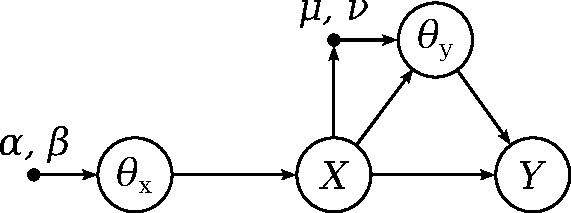
\includegraphics[scale=0.5]{2var_2param_4const}
	\caption{Two correlated random variables, $X$ and $Y$, with their probability mass functions parameterized by $\theta_\mathrm{x}$ and $\theta_\mathrm{y}$, which are themselves random variables defined through their respective hyperparamters $(\alpha, \beta)$ and $(\mu, \nu)$.}
	\label{fig:2var2param4const}
\end{figure}

Without going through every step of our derivation again, we list here only how introducing hyperparameters changes a few key formulas.

\section{Bayesian hypothesis test}
Suppose $X$ is a binary random variable, representing if a patient has recieved a certain treatment or not, and $Y$ is also binary random variable, indicating whether patient's symptoms disappeared or not. Our goal is then to learn the distributions of the parameters, $\theta_\mathrm{x}$ and $\theta_\mathrm{y}$, describing the probabilities of $X$ and $Y$ occurring, respectively.

As we are dealing with binary variables, we can chose between a \emph{Beta-Bernoulli} and a \emph{Beta-Binomial} model. As the names imply, the priors on $\theta_\mathrm{x}$ and $\theta_\mathrm{y}$ are \textit{Beta} distributions in both models, each characterized by two parameters.


\chapter{Good Things Come in 3's}
Example binary classification

\chapter{Continuous Variables}
Density vs. mass function and the mystery of observation and hidden variables.

\end{document}          